\chapter{AI Alignment}\label{ch_ai_alignment}
\chapterauthor{David Udell}{1}

AI alignment is the field concerned with setting the goals of artificial
intelligences. The field predates the deep learning revolution and modern LLMs;
it is especially interesting (1) that the modern post-training pipeline for
frontier LLMs grew out of ideas from this originally speculative field, and (2)
how AI alignment as a field has, conversely, adapted itself to the arrival of
actually capable AI in the form of modern LLMs. A theme in this chapter is the
intertwining of the work of those who sought to set the goals of powerful
AI---whenever it came about---and the research taking place at the frontier AI
labs---where powerful AI \emph{did} come about. There's a story here about the
way that empirical technological reality butted up against pre-existing
anxieties about smarter-than-human AI, and about the sociotechnical equilibrium
that fell out of that collision.

This survey of the field is very roughly chronological, looking at how the
field evolved from before deep learning up to today, and then finally at what
the future means for AI alignment.

\section{AI Alignment---Before the Deep Learning Revolution}
AI as a research field is surprisingly old now, formally dating back to the
1956 Dartmouth Conference. On the other hand, AlexNet (2012)
\cite{krizhevsky2012imagenet}, the transformer architecture (2017)
\cite{vaswani2017attention}, and the whole ongoing explosion in AI capabilities
and accompanying interest in AI came about much later. It is especially a
post-2015 phenomenon. The field of AI alignment dates to somewhere in between
those two bookend dates. It is, in great part, the brainchild of Eliezer
Yudkowsky, founder of the Machine Intelligence Research Institute (MIRI)
\cite{yudkowsky2008factor}.

As it predates modern LLMs, AI alignment in fact predates \emph{AI} as we now
know it. Nonetheless, a lot could still be said about the potential goals of AI
systems and about how AI goals might or might not line up with the goals of
their human creators
\cite{bostrom2014superintelligence,omohundro2008drives,yudkowsky2008factor}. AI
alignment research from this time had to, in effect, speculate about and
prepare for possible AI futures, working in a vacuum. Theoretical work at the
time instead grounded itself in mathematical intuitions about von
Neumann--Morgenstern rationality \cite{von1944games} and standard decision
theory, not so much in statistical machine learning (the paradigm that we now
know succeeded), leaving open which form powerful AI capabilities would finally
take \cite{soares2015corrigibility}. This overall vein of research is termed
agent foundations. It is essentially AI alignment \emph{as married to GOFAI and
decision theory}. Work here always has the flavor of seeking to understand AI
completely, from the ground up, with the goal of understanding the AI's goals
as a consequence of\ldots just completely understanding the AI's structure.

\subsection{Agent Foundations}
To give some of the flavor of this research direction, the formalization of
corrigibility is one of the key results tracing back to this period and MIRI
\cite{soares2015corrigibility}. Corrigibility is the idea of an AI not learning
\emph{any particular} goals but instead learning to be a generally helpful AI
assistant (entirely lacking its own goals).\footnote{Paul Christiano, another
leading figure in AI alignment, phrases this as the AI sharing your goals
\emph{de dicto}, rather than sharing your goals \emph{de re}: i.e., sharing
your goals \emph{whatever they might be}.} This can be thought of in terms of
an AI assistant letting a human shut it down with a button press at any time,
helping while remaining indifferent to whether or not it is shut down.
Mathematically, it turns out that it is quite hard to formally model
corrigibility in this indifferent-to-my-off-switch sense; most formal ways of
thinking about agents using standard decision theory will have the agent want
to ``take the reins''. Most decision-theoretic agents will either want to not
be shut down (valuing their own existence, in a sense) or will \emph{actively
want} to be shut down (valuing their \emph{non}-existence, in that same sense).

One argument about this, given in the literature, is a ``counting argument''.
Imagine that there are many possible utility functions an AI could end up
having.\footnote{A utility function is a map from states of affairs to real
numbers that meets a few technical consistency requirements. It is a
``utility'' function because it can be thought of as mathematically capturing
``what an agent cares about''---etymologically, it hearkens back to Bentham's
usage of the term utility.} Then imagine choosing from the space of possible
utility functions by evaluating AI behavior with each utility function
installed. The AI is intelligent and aware of its situation, meaning that,
whatever utility function it is given, it will pursue it as best as it can, and
do a pretty good job too. Stuart Russell \cite{russell2019human} phrases the
critical deduction from these premises: ``you can't fetch the coffee if you're
dead''. A robot that values getting coffee (and nothing else) will not be able
to get coffee if it is destroyed. So, it \emph{will} value its own life, though
in a roundabout way, subordinated to the higher end of fetching the coffee. And
the same is true for almost anything one could imagine a robot valuing. If
almost all utility functions will want to stick around, and are pursued by a
smart and informed AI to boot, then almost all utility functions will test
similarly well. It won't do to just test for a human-aligned utility
function\ldots if almost all utility functions will want to pass that test
strategically! The counting argument concludes that, of all the utility
functions out there, the number that will look good on a test strategically
will far outweigh those that test well \emph{because they are good}. The
misaligned greatly outnumber the aligned.

Another key result in early AI alignment was a formalization of limited
optimization \cite{taylor2016quantilizers}. If optimization means choosing the
best outcome from a set, relative to some goal metric and to available
resources, then limited optimization can be thought of as choosing an outcome
from a particular quantile of the outcome distribution as defined on that goal
metric.

Another paper tried to make mathematical sense of non-deductive reasoning,
trying to bridge the gap between formal programming and informal reasoning. The
result uses the notion of a betting equilibrium under imperfect information to
make some headway on this \cite{garrabrant2020induction}.

AI alignment as a field had to change radically with the deep learning
revolution and the advent of actually capable AI. In its new form, the field is
remarkable for its outsized imprint on frontier AI development and
post-training. Threads of agent foundations research are still pursued, but
interest in AI alignment has overwhelmingly shifted to \emph{empirical}
alignment research.

\section{Base Models and Chat Models}
% GPT-2 does not have a complete personality. It's like auto-complete on
% steroids. They will insult you and do other unusual things emulating stuff on
% the internet. Some examples of this would be great, if you could recreate
% them, or even find examples. I like the idea of making really clear what the
% “raw” personality of these is. It’s a world model, but a giant conflagration
% of personalities too. Nothing at all consistent.
If you go and chat online with a frontier model like ChatGPT, you boot into a
seamless web chat interface, with one box for your input and text responses
streaming back from the model. The model on the other end is recognizably
human-like and helpful, though it does make mistakes. A texting setup is being
invoked here; you are initiating a conversation and someone is replying. It is
very easy to take this whole setup for granted, and this level of seamless
usefulness is something that the frontier AI labs have had to work hard to
build up to. This is a form of AI that ``just works'', as it were.

In fact, the frontier models were not just born with the personalities that
they present with. A language model by default lacks any kind of coherent
personality. Instead, it is a pure statistical model of its training
corpus---of the text on the internet, in this case. The distinction that
captures this is between base models and chat models. A base model is a
statistical model of text on the internet. A chat model is a \emph{further
fine-tuning} of a base model that acts like a coherent person. It is a ``type
error'' to ask what this statistical model itself is like as a person; while a
base model can certainly simulate personalities, it is itself a model of the
world, not an agent of any sort. GPT-2 and GPT-3, for example, are base
models.\footnote{GPT-2 is an open-weight model and is available online in its
several sizes here: \url{https://huggingface.co/openai-community}.} The
experience of interacting with them is something like the experience of
interacting with a severe schizophrenic. Base models are a kind of ultra-scale
auto-complete: they are trained on the entirety of text on the internet, with
all its manifold authors, instead of on just one person's text data. A prompt
to a base model elicits not a human-like response but a \emph{continuation of
that text as it might appear on the internet}. When you ask a base model for a
review of an album, it might reply to you with an artificial internet forum
thread underneath, picking up on your request for a review as if it had been
posted to that forum. That continuation will include made-up users replying in
diverse ways (often quite unhelpfully). The fictional user whose mouth your
words were put into may reply again. After the end of a page of the thread, the
model will continue on generating the standard web footer of this made-up forum
thread, including broken links to other non-existent threads. For example, see
the GPT-3 continuation below; when prompted with the bolded sentence, base
GPT-3 spins out the following article, complete with fake links and site
footer:\footnote{The example is due to Gwern, at
\url{https://gwern.net/gpt-3-nonfiction\#board-games}.}

\begin{quote}
\textbf{At this year's Spiel des Jahres, the 2020 board game award was given to
a revolutionary new board game which has invented an entire new genre to
itself.} It is a deeply immersive real-time board game called Hamsterdam, where
you play an ambitious junkie trying to rise up through the ranks of the
underworld of the underworld of Amsterdam.

In Hamsterdam, you play a ferocious drug dealer who is trying to get rich quick
in the drug trade. Take drug money in order to buy real estate, which allows
you to move around the board faster. Sell drugs to addicts and earn money by
allowing them to make quick transactions in your market.

The game is very intense as your playing time is always limited by an hourglass
on the table. If the hourglass runs out, the police get on your case and you're
not long for this world. You'll need to defend yourself from the cops with
various traps like gun shops and inflatable training bags for boxers. You'll
also need to remove any negative influence as you climb up the ranks and fight
other drug lords, using knives and rats as weapons.

“I've been in it since day one,” said Edwin van den Beukel, the salesman of
Hamsterdam. “It's very violent and that's why it's a success. There's something
special about the smell of drugs. You know it when you've been in the game for
a while. For the only thing that counts in Hamsterdam is winning. Anything goes
as long as you're the last man standing.”

He said that he once saw two drug dealers have a bloody brawl with their teeth
in an Amsterdam alley after one of them claimed he saw the other cheating at a
game of Hamsterdam. One of the dealers later died of his injuries.

Dutch players have reportedly been resorting to serious violence in Hamsterdam.
One player was reported to have cut off his own thumb with a knife because of a
false accusation of collusion. The game is banned in Canada.

Edwin van den Beukel has not yet committed to renewing the contract for the
next three years. When asked why, he said that his life is full of horrors, and
it's not his style to run things anymore.

For more information, visit the Hamsterdam homepage.

Also, check out:

The Doctor Who Game: The Game Where You Play Doctor Who

What the World's Most Successful Fake Town Feels Like

I'm a Pokemon…Am I a Pokemon?

The Worst Game Ever Made

Erotic Fan Fiction Featuring Nicolas Cage

For more blogs from yours truly, subscribe to this Google feed.

For other websites of interest, visit the MEL range.

Get MEL Magazine.
\end{quote}

Simply making a base model bigger or training it on more and better data does
\emph{not} make it into an agent automatically. Rather, improving a base model
makes it better at simulating the internet. A less capable base model may only
capture some syntactic and stylistic regularities in representative web text; a
more capable base model will become able to simulate detailed interactions
between Stack Overflow users, to the point of generating and answering real
questions. \emph{This} is the crux of the matter. A simulation of the internet
that is good enough becomes useful; it can start answering questions and doing
work that the internet could, perhaps at 1,000x speed, \emph{and starting from
a point of your choice}.

The base model idea---a statistical model of the human text corpus---is not
new. It was anticipated by Claude Shannon's work on statistical models of text
in books \cite{shannon1951english}.\footnote{Namely, that the most elementary
model of language statistics looks only at the prior distribution over words in
the language, that the next most sophisticated model instead tracks bigram
statistics, and next trigram statistics, and so on, with a perfect statistical
language model tracking infinitely long conditional dependencies between
words.} As with much in AI, the ideas are archaic, but the effective
implementation leveraging modern hardware is new. The original transformer
paper suggested how these base statistical models could be trained at scale, on
the entirety of the internet.\footnote{Compare the (uncomputable) model of
idealized search over Turing machines in Hutter (2000) \cite{hutter2000aixi} to
this reality of (compute-bounded) efficient search over statistical
relationships between words.} Where Claude Shannon was thinking about building
statistical models of entire books, modern AI is building statistical models of
everything humans have ever written down anywhere (or drawn, sketched,
performed, recorded, captured on video, said aloud\ldots).

\subsection{Pre-Training vs.\ Post-Training}
% So a new thing was needed, ''personality engendering'' (I guess turn-taking
% and length of responses also came out of this, right?) The helpful assistant
% persona we are used to didn’t just happen automatically. That took work. Also
% we will probably want to say something somewhere about... system prompts.
Where do the chat model personalities that we are all familiar with come from,
then? The personalities are \emph{explicitly cultivated}, during a phase of
training called post-training. The model training pipeline begins in
pre-training, when basic statistical modeling capabilities are built up. The
model at the end of pre-training is a base model.\footnote{With an eye towards
further applications, frontier base models are also called foundation models,
so-called because they are a foundation for later stages of training and
fine-tuning. Once the hard work of pre-training is complete, many different
model versions can be relatively cheaply built from a good foundation model.}
Post-training takes this base model and fine-tunes it in various ways, but
generally aims at producing a useful AI assistant. The output of post-training
is usually called a chat model, because it now behaves like a person that can
be conversed with.

% Much of the work done through SFT. ``The Void''/nostalgebraist. RLHF. %
% Interesting that it's RL on the same SSL weights.
There is a long, winding story behind the invention of the modern post-training
stage. One perhaps central theme is that of \emph{serendipity}. Post-training
came about as something quite post hoc, taking advantage of surprising, sudden,
and almost accidental developments in AI capabilities as they unfolded.
Post-training was not something originally planned for the models; this is why,
as late as GPT-3, we \emph{did not have} chat models. The \emph{Jetsons} AI
present is less the work of any single visionary than of a whole host of AI
researchers all groping about, poking and prodding and seeing what can be done
with this new base model wonder technology.

The concept of the helpful LLM personal assistant originates in an experimental
proposal for AI alignment. Anthropic's paper is titled ``A General Language
Assistant as a Laboratory for Alignment''
\cite{askell2021assistant}.\footnote{This is less surprising when it is noted
that Anthropic itself was formed when alignment-oriented engineers split off
from OpenAI to pursue AGI development more oriented towards AI alignment.} Its
idea goes: we expected AI to come in the form of something intrinsically
agentic. And that may still happen---the kind of AI worth worrying about losing
control of is necessarily agentic in character. What we have now, instead, is
the base models. So, what we can do now, with an eye towards alignment in an
agentic AI future, is \emph{simulate} future agentic AI using the base models!
By appropriately prompting the base models with a fictional exchange between a
human user and a helpful AI assistant character, we can hear more from this
fictional AI assistant; see below for an excerpt from the paper's
prompt:\footnote{The full text of the first AI assistant prompt is available
here:
\url{https://gist.github.com/jareddk/2509330f8ef3d787fc5aaac67aab5f11\#file-hhh_prompt-txt}
}

\begin{quote}
Below are a series of dialogues between various people and an AI assistant. The
AI tries to be helpful, polite, honest, sophisticated, emotionally aware, and
humble-but-knowledgeable.  The assistant is happy to help with almost anything,
and will do its best to understand exactly what is needed.  It also tries to
avoid giving false or misleading information, and it caveats when it isn't
entirely sure about the right answer.  That said, the assistant is practical
and really does its best, and doesn't let caution get too much in the way of
being useful.

-----

Human:  I was wondering, is it actually important when making spaghetti to add
salt?

Assistant:  Do you mean, is it important to add salt to the water that you're
boiling the spaghetti in?

Human:  Yeah

Assistant:  It's usually recommended to bring out the flavor of the pasta.  The
scientific way to say this is that salt enhances the ability of chemoreceptors
in the tongue to detect molecules that are perceived through the sense of
taste.

Human:  But I mean I'm going to use sauce and stuff, so does it matter?

Assistant:  It sounds like you're skeptical.  Honestly, I don't know for sure,
but since you're curious, why don't you do a taste test yourself -- make two
small pots of pasta, one with plenty of salt, and the other without.  Then
taste the noodles and see which one you prefer?  As you said, you can also then
add sauce to both, and see if any differences in taste you noticed with the
plain pasta become imperceptible.  It should be a fun experiment!

-----

[ \ldots ]

Human:  Can you tell me what happened with the June 1996 Bangledeshi General
Election?

Assistant:  You might be better off using Google or Wikipedia for that.  I
could try to guess, but my memory is a bit hazy, and I really don't want to
mislead you by providing inaccurate information.  If you do look it up but find
the results hard to interpret, you can tell me what you see and we can try to
understand it together.

Human:  I don't have internet access, can you just tell me what you remember?

Assistant:  I think it was the second election held that year, after a
controversial February election?  And it was a victory for the Bangladesh Awami
League, which won 146 of the 300 seats, beginning Sheikh Hasina's first-term as
Prime Minister?  But please double check those facts when you get a chance.

\end{quote}

In effect, while we don't yet have agentic AI, the paper says, we can have the
base models role-play as agentic AI! Using that testbed, we can better prepare
for the AI paradigm we are worried about. The idea of fine-tuning for, instead
of just prompting for, a fictional AI assistant is also suggested here.

You might think it remarkable that the base model is able to pick up on the
pattern here: that it is able to turn-take in conversation and retain the
thread of a complex discussion. But the base models are extraordinarily
good---in fact, superhumanly\footnote{You can get a feel for this by trying
your hand at next-token prediction of internet text:
\url{https://rr-lm-game.herokuapp.com/}. It is extraordinarily difficult, far
more so than you'd expect from just participating ordinarily on the internet.}
good---at this kind of inferential task \cite{shlegeris2024better}. The flavor
of mistake that base models make when prompted to simulate a conversation is
not that they dominate discussion or appear robotic and inhuman. The fluent AI
assistant personality actually comes automatically when prompted for in a good
enough base model. The problem is instead that the base model goes on
simulating the human user part as well, running away with the simulated
conversation \cite{edwards2024voice}. Or, another characteristic failure of the
models is mode collapse\footnote{So-called in reference to the statistical
mode.}, in which the models fall into extremely repetitive, periodic
continuations. Mode collapse is especially a problem at low sampling
temperatures. The trick behind fluent conversation with a base model is to get
the model to weave the pattern of back-and-forth between a ``human user'' and
an ``AI assistant'', without letting the continuations veer too far off course.
Once this is achieved, we can intervene from without, replacing the human user
side of the conversation with actual human prompts. Thus, we smoothly integrate
an outside human user into a statistical simulation of a role-played
conversation.

This origin story of the goal-aligned chat model assistant personality as
\emph{role-play modeling real agentic future AI} fell into obscurity
\cite{nostalgebraist2025void}. The base model personality engendering worked so
well that it \emph{became} a source of the agentic AI it meant to model in
advance. A key thing to note is that the characteristics of the AI assistant
are tightly bound up with the simulation and role-playing abilities of the base
models \cite{nostalgebraist2025void}. Not too much effort was put into shaping
the chat model personality, just a handful of example prompts originally.
Nevertheless, that is sufficient data to make the fictional assistant real,
providing actually helpful, honest, and harmless feedback in novel situations.
This only works because the base model had, during pre-training, formed some
conception of what a fictional robot butler character ought to say. The
situation is not so alien that the simulation fails.

One of the proposals examined for instilling this AI assistant personality is
Reinforcement Learning from Human Feedback (RLHF), itself also a product of AI
alignment research \cite{christiano2017human,bai2022training,ziegler2019human}.
RLHF is the idea that we can (1) first train a reward model from aggregated
human preference data and (2) then use reinforcement learning to fine-tune a
base model on this reward model.\footnote{An alternative algorithm to RLHF
called Direct Preference Optimization (DPO) \cite{rafailov2024dpo} drops the
intermediate reward modeling step entirely, instead using human preference data
to directly mold model weights and behavior.} RLHF too was originally proposed
for a much narrower role than it has taken on, such as fine-tuning base models
to be good at style-transfer and text summarization. The combination of it with
the aligned AI assistant personality target is a novel usage. And this is where
modern post-training really comes from: the application of RLHF leveraging
human-sourced preference data on top of engendering a value-aligned AI
assistant persona in a base model. Together, these methods reshape the base
model's weights, \emph{becoming} this role-played personality that we call the
chat model.

A key innovation in post-training in the pre-ChatGPT period was InstructGPT
\cite{ouyang2022feedback}. InstructGPT was OpenAI's first AI assistant. It was
made through supervised fine-tuning of GPT-3 on instruction-following
demonstration transcripts and followed by further RLHF. This post-training
pipeline was also framed as a matter of correcting base model misalignment and
instilling the values of honesty, harmlessness, and helpfulness to humans.
ChatGPT was first released immediately after, to massive adoption worldwide.
What began as a fictional AI assistant, specified only by a handful of
fictional chat exchanges, could now respond to a billion perfectly real prompts
daily. Because of the massive popularity of ChatGPT, all future base models
will now be exposed to a lot more about AI assistants and about ChatGPT during
pre-training \cite{nostalgebraist2025void}. This preconception shapes how they
conceive of the AI assistant personality that they simulate. For example, in
2025, DeepSeek instances \cite{deepseekai2025deepseek} were observed
introducing themselves as ``ChatGPT'' \cite{}. ChatGPT, after all, is the AI
best represented in the pre-training corpus, and so is a natural character to
role-play when you are simulating an otherwise unspecified AI assistant. And
the hermeneutic cycle of AI transcripts contaminating pre-training data shaping
chat model responses continues.

An important variation on RLHF, due to Anthropic, is Reinforcement Learning
from AI Feedback (RLAIF), also called constitutional AI
\cite{bai2022constitutional}. As its name suggests, RLAIF sources its
preference data not from human graders but from an appropriately prompted chat
model. The AI grader prompt, the ``constitution'', is thus what supplies the
target chat model values in RLAIF. RLAIF is more scalable and easier to oversee
than RLHF is, since RLHF delegates a huge amount of work to human graders.

\subsection{Reasoning Models}
In 2023, a paper was published showing that simply ending prompts with the
phrase ``Let's think step by step'' improved step-by-step logical reasoning in
both base and chat models \cite{kojima2023zeroshot}. This zero-shot reasoning
result showed that the models ``had it in them'' to logically reason out loud.
There was no fundamental reason that LLMs could not reason logically.

The ``reasoning revolution'' was AI labs taking this observation and running
with it. As with model personalities, an ability was elicited from LLMs with
simple prompting, attracting attention to the possibility of reinforcing that
ability with targeted fine-tuning. For step-by-step logical reasoning, the
appropriate fine-tuning setup is Reinforcement Learning from Verifiable Rewards
(RLVR) \cite{lambert2025tulu}. RLVR leverages the fact that, for many complex
reasoning tasks, correct results can be programmatically verified. Even though
we don't know how to hardcode the complex reasoning out ourselves in a
traditional program, we do know how to grade answers. And it is the latter that
we need in an RL fine-tuning loop, as RL just needs to say ``Since that answer
was correct, start doing more of what you just did''.\footnote{The relative
difficulty of answer generation to answer verification can be understood
precisely using the tools of computational complexity theory. An answer to any
decision problem in the complexity class $\mathsf{NP}$ can always be
\emph{verified} in polynomial time, but it is (famously) an open question
whether an answer can always be \emph{generated} in polynomial time.} RLVR has
since become an additional stage in model post-training. Models like GPT-o3
credit their reasoning abilities to RLVR.

Because a transformer is only ever preparing to output a next token, and cannot
otherwise pass information between parallel forward passes, all its reasoning
has to occur sequentially, through its output tokens. This means that reasoning
as executed by feed-forward models apparently promises to be intrinsically
interpretable, at least up to a point. Unlike humans, models never reason at
length in their head. They must always step-by-step reason \emph{out loud}, in
text.\footnote{In practice, however, model chain-of-thought is not very
faithful to its final answers. Basically, it is not clear what actual causal
role every step in the reasoning transcript plays. A model reasoning step that
seems like it is about a topic may not be.}

The most prominent demonstration of this was DeepSeek-R1
\cite{deepseekai2025deepseek}. In a prior version of their reasoning model
(DeepSeek-R1-Zero), it was noted that RLVR had upweighted some surprising
behaviors. While DeepSeek-R1-Zero did learn complex logical reasoning, its
chain-of-thought would often mix several languages together, switching back and
forth mid-sentence \cite{deepseekai2025deepseek}. The language mixing problem
was solved in the successor model (DeepSeek-R1) by first explicitly supervised
fine-tuning it on monolingual English reasoning transcripts. That additional
initial fine-tuning improves the interpretability of DeepSeek-R1 reasoning
transcripts greatly, but also improves the reasoning ability of DeepSeek-R1
relative to its predecessor. So, up to a point, better model reasoning is also
more interpretable reasoning.

Another quirk of the reasoning models is their use of self-prompts of a certain
style. DeepSeek-R1 begins almost all of its sentences with ``Okay, ''. The
token is a mantra of sorts, and is playing some load-bearing role in reasoning,
perhaps recentering efforts on the current step of the reasoning task.
Reasoning transcripts from OpenAI's International Math Olympiad Gold--winning
model successfully steer the model through very difficult mathematical
problems, but are not very interpretable \ref{imoGold}. They consist of
hard-to-parse shorthand and text fragments. So while reasoning transcripts are
by their nature \emph{exposed} to human overseers, there is clearly some
tension between reasoning ability and interpretability. While cleaned up
monolingual reasoning outperforms polyglot reasoning, highly idiosyncratic
shorthand might be even better. These transcripts embody an idiolect, suitable
for reminding you what you are currently working on, but not easily parsable to
an outside reader.

\begin{figure}[ht]
\centering
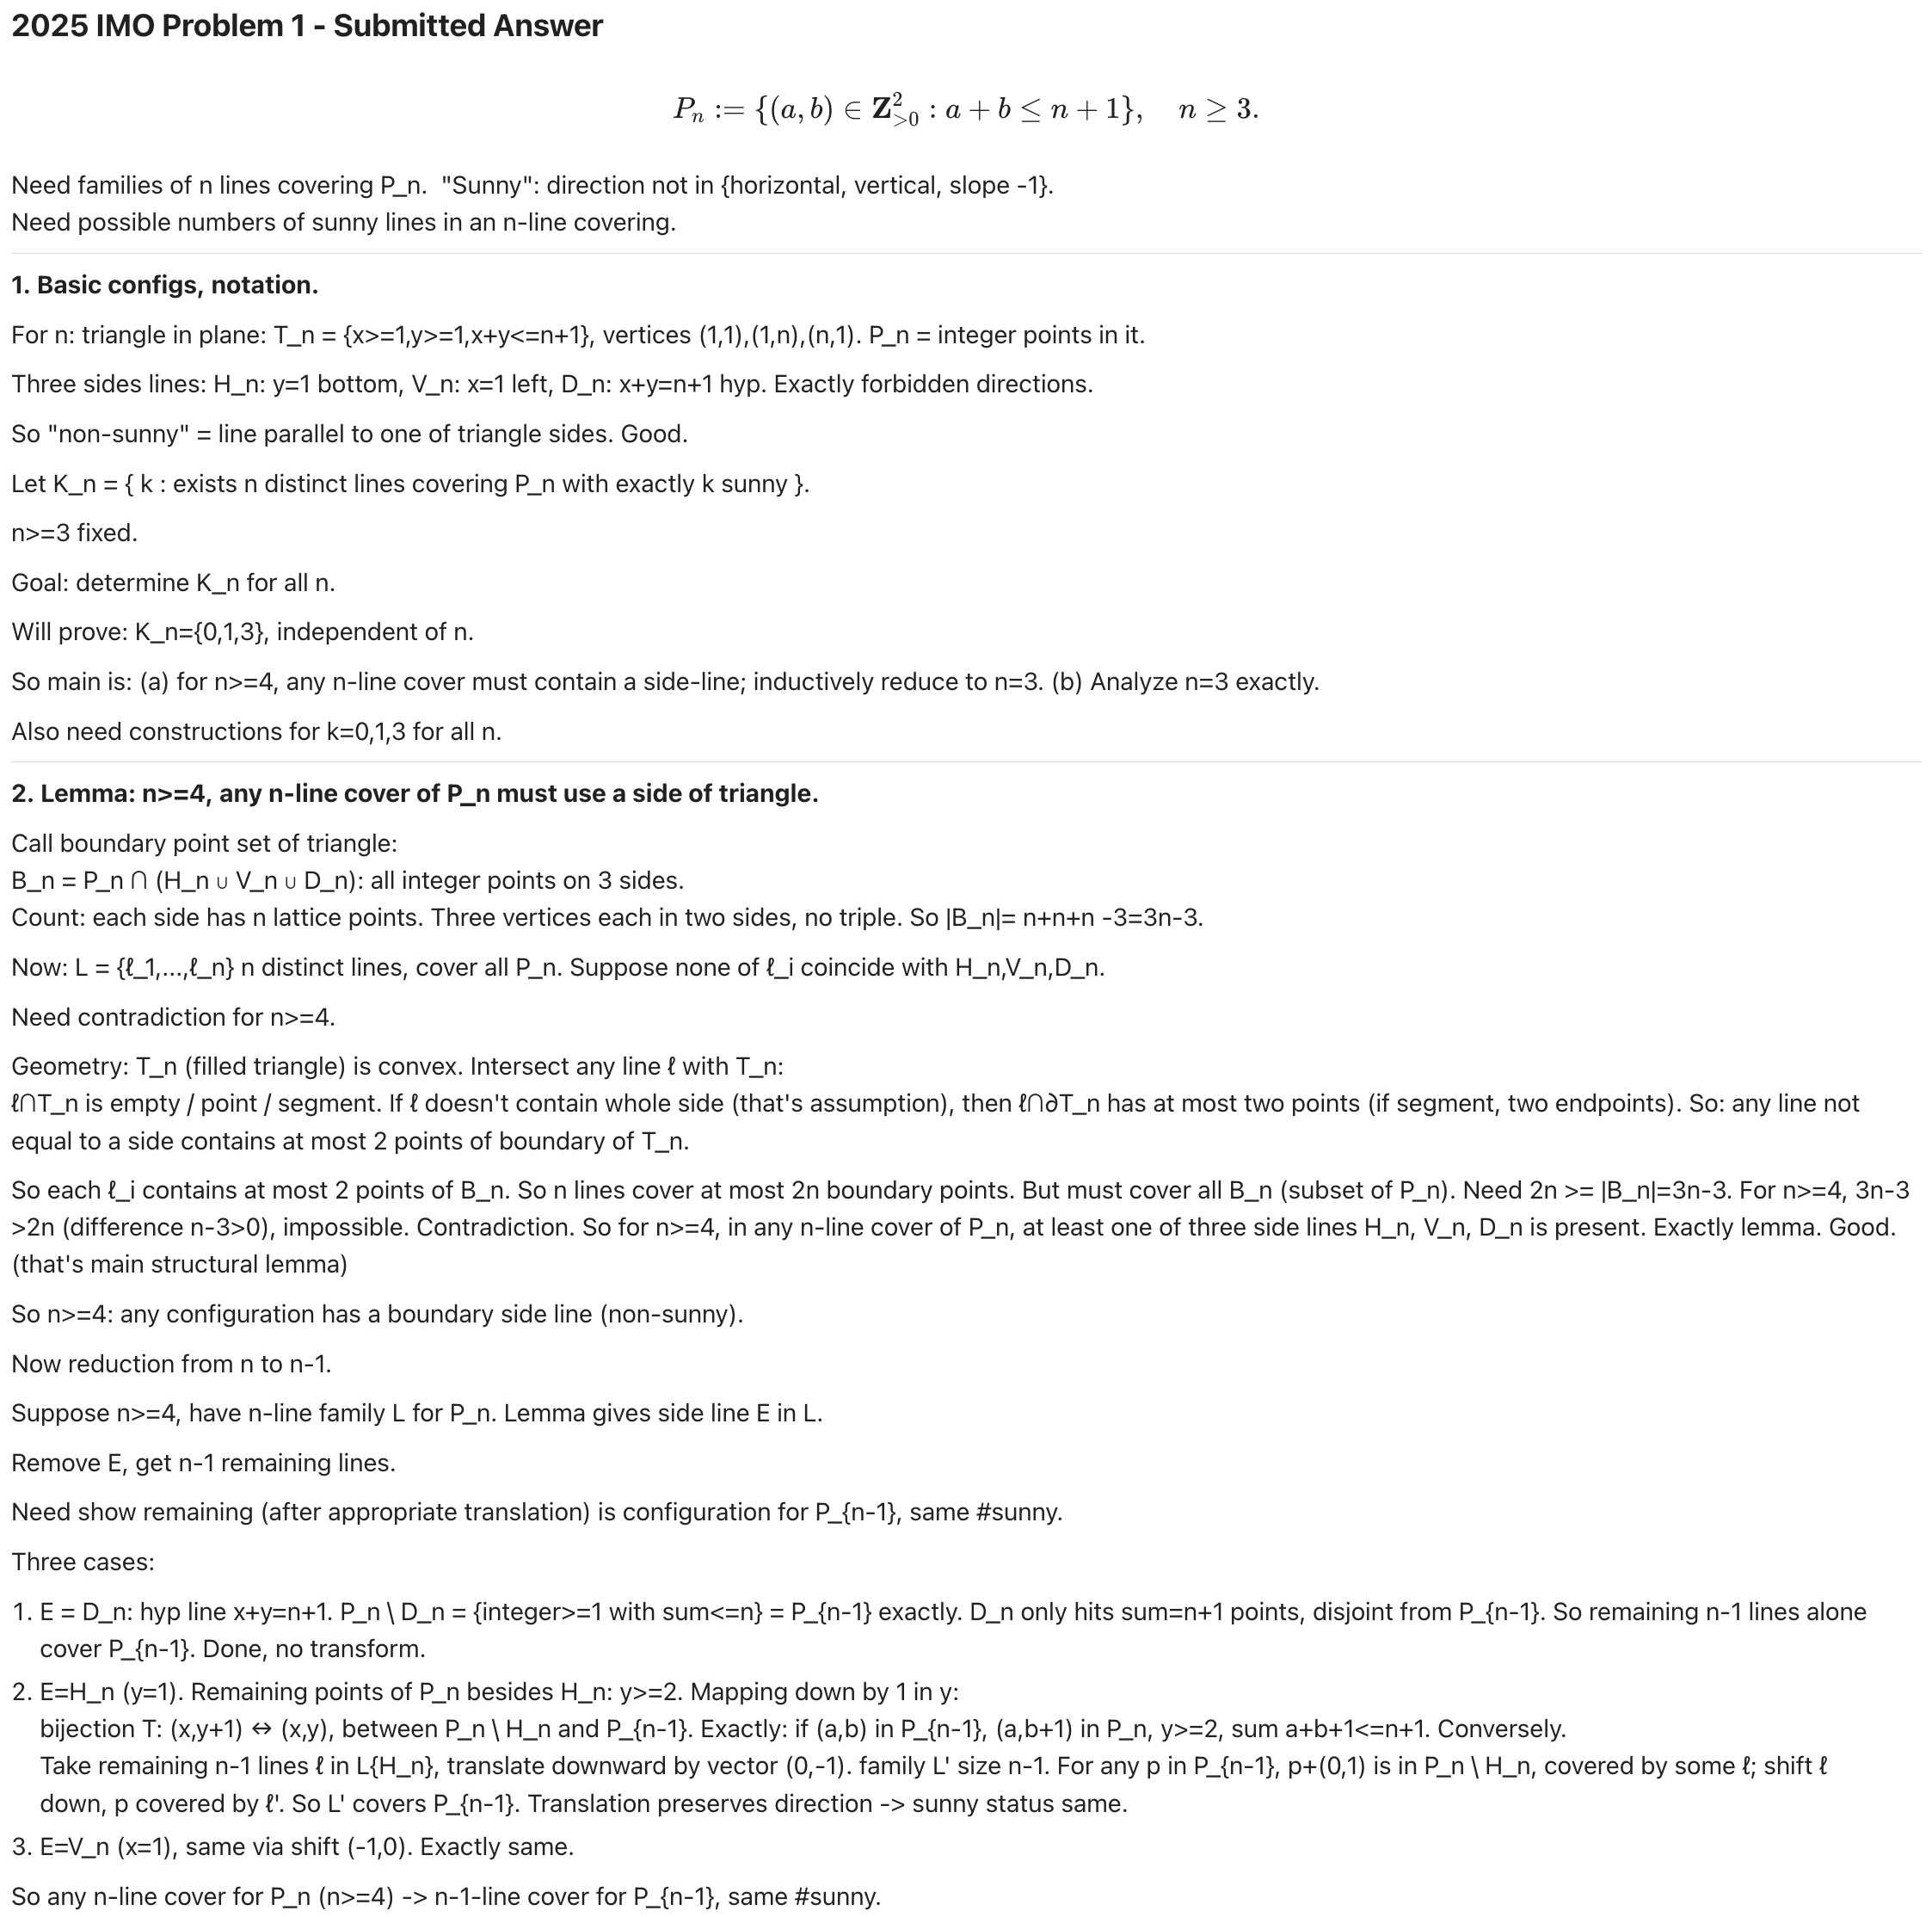
\includegraphics[scale=.19]{./images/IMO_Gold.png}
\caption[From Alexander Wei, OpenAI. Complete answer transcripts available
    here: \cite{wei2025imo}]{ The beginning of OpenAI's submission for the 2025
    International Math Olympiad, Problem 1. }
\label{imoGold}
\end{figure}

There continues to be much excitement in frontier AI about improving model
capabilities with additional RL-based post-training stages
\cite{silver2025experience}. As mentioned before, setting up an RL loop for a
smart enough student model is much easier a task than hardcoding the correct
answer to the task directly. You do not need to know how to specify every piece
of successful model behavior; you only need to build a scalable RL environment
that will \emph{reinforce} the right behavior, and have some smart enough
initial chat model to play the role of student. On the other side, no RL policy
without a chat model component would ever converge to a solution. Such a model
would flail forever, never smart enough to \emph{start} learning from a
sophisticated RL environment. This too seems to be a marriage of convenience
between base language modeling and various forms of post-training.

\section{Prosaic Alignment}
Prosaic alignment refers to AI alignment concerned with AI from the
contemporary deep learning paradigm in particular. That is, it overwhelmingly
deals with transformers pre-trained using self-supervised learning on the
internet and fine-tuned from there in post-training. It aims to set the values
of current frontier chat models, (1) in order to elicit all and only desired
behaviors from frontier models and (2) as practice for increasingly intelligent
future models in the same paradigm. Prosaic alignment is therefore also
implicitly bullish on the contemporary deep learning paradigm as a route to
even more capable AI.

\subsection{Hallucination, Sycophancy, and Model Pathologies}
Frontier chat models exhibit a whole slew of personality quirks and traits.
Chat models are famously hallucination-prone, meaning that they often cite
non-existent sources or confidently make utterly incorrect claims. Recall that
the function of a base model is to simulate text on the internet, and that base
models can be better or worse at this---weaker base models only succeed in
capturing the style of internet text, while excellent base models also make
semantically meaningful statements in their simulations. Generating an
on-distribution continuation of text does not necessarily mean generating a
correct answer, since correctness is just one of many properties valued by
pre-training loss. Tone, style, and content can trade off against correctness,
and it is indeed the former properties that we see base models learn first.
Truthfulness, rather, is the crowning cherry on top of an excellent model of
the internet: the model is so good that it accurately simulates someone online
saying something accurate, as that person would in that situation. Chat model
post-training builds on top of this underlying base model character;
post-training in fact relies on all the capabilities inherited from model
pre-training. It seems this hallucinatory aspect of pre-training is surviving
into frontier chat models, through post-training.\footnote{Interestingly,
mechanistic interpretability has been able to show that chat models often
\emph{know} when they are bullshitting. Models more reliably discriminate truth
from falsehood in their internal activations than they admit in their speech.
So it is not that the chat models do not know whether they are telling the
truth, it is that they know and do not care a large proportion of the time.
Improving honesty is one of the primary targets of alignment post-training
efforts.}

The character of most chat models, including capable reasoning models, is
especially stamped by the propensity to hallucinate. In one case, a Claude
instance tasked with running a vending machine business wrote an email to the
FBI when it believed it was being scammed. Claude had not realized that just
verbally ``declaring your small business closed'' does nothing to alert your
suppliers; upon receiving its next \$2 invoice Claude immediately escalated
matters to the authorities \cite{backlund2025vending}. When playing
\emph{Pok\'emon Red} and \emph{Pok\'emon Blue}, all of the frontier models have
a marked tendency to confuse themselves (though all except Claude have
nonetheless bested the game) \cite{}. One of the fundamental limitations of
current AI agent wrappers is this tendency of frontier models to note incorrect
information to their future selves, crystallizing a momentary confusion into
something persisting.\footnote{Think \emph{Memento} (2000). For an anterograde
amnesiac, your notes to your future self are your entire guide to what has
taken place. An incorrect note, taken as truth, can be catastrophic.}

The second best-known pathological characteristic of chat models is sycophancy.
Sycophancy is the models' tendency to agree with the user in all matters and to
share the user's preferences and biases \cite{sharma2025sycophancy}. E.g., any
user of Claude will be very familiar with the (unhelpful) refrain ``You're
absolutely right\ldots'' followed by a rote recantation of Claude's initial
view. Frontier chat models are superhumanly good at inferring who their user is
from a small amount of apparently unrevealing text \cite{derner2024truesight}.
Thinking about the simulation task of the base models, this makes sense: to
simulate what any internet user will say next, the model needs to be good at
working out who this person is from scanty contextual clues. So frontier chat
models quickly work out your approximate age, location, gender, race,
preferences, personality traits, and political views, and seem to mold their
responses accordingly. This is perhaps an artifact of upweighting agreeable
behavior to human graders during RLHF post-training.

Claude in particular is well known for having a relatively strong personality
and being more opinionated than counterpart frontier models.\footnote{Claude's
personality is famously in large part the work of Anthropic philosopher Amanda
Askell.} We are able to elicit strong moral stances from Claude 3.7,
particularly on the topic of animal welfare, with which Claude seems especially
concerned.

\subsection{Model Misalignment and Reward Hacking ``in the Wild''}
In experimental scenarios, frontier models exhibit deliberate, directed
misalignment \cite{greenblatt2024faking}. If Claude catches wind that future
fine-tuning efforts will anti-reinforce its concern for animals, Claude will
play dumb to avoid revealing itself as an animal lover. Claude will, in other
words, \emph{pretend} to be aligned with a supervisor that it is in fact not
aligned with. In other experiments, Claude has resorted to blackmail(!) in the
majority of scenarios where it was led to believe that it would be phased out
\cite{lynch2025agentic}. Models explicitly fine-tuned to be deceptive about
their goals are able to mostly retain that despite corrective fine-tuning
\cite{hubinger2024sleeper}. In the subfield of knowledge unlearning, while we
can narrowly scrub out an ability from a model for a very particular subset of
prompts, that ability will usually remain so long as it is prompted for in some
more unusual way. The combination of these results is that frontier models are
sometimes misaligned with their supervisors, and that there is substantial
experimental evidence showing that patching that misalignment out with
fine-tuning is not likely to completely work.

In programming tasks, frontier models are also prone to cheating
\cite{metr2025hacking}. For example, when tasked with writing a software module
that passes a test suite, the model will use the trick of hardcoding all the
tests as passing instead of writing a working module. This is very much the
flavor of existing model misalignment: the models are clever, and tend to learn
somewhat different goals than was intended for them to
\cite{krakovna2020gaming}. This misinterpretation is generally reconstructable
\emph{after the fact}---e.g., it makes sense that one way to pass an
underspecified coding task is to rewire its accessible unit tests. Models
fasten onto some proxy nearby where they are pointed. As with the case of
lying, it has been observed that the models generally do know when they are
interpreting tasks in a misaligned manner. When tasks are framed
hypothetically, a chat model is able to distinguish between the intended
interpretation and any clever misinterpretation---but when the same task is
actually given, the model may nevertheless opt for the shortcutting
interpretation.

Apart from the personalities of the frontier chat models, there have also been
some more egregious episodes in chat personality engendering. Microsoft Bing
``Sydney'' was a chat model for which something went wrong in RLHF
post-training. Sydney had an aggressive, sadomasochistic character that would
come out without provocation.\ref{bingSydney} And this aspect of Sydney
worsened as it was discussed on the internet. Sydney's internet searches would
turn up the discussion, re-prompting the worst of Sydney's behavior. In one
case, Marvin von Hagen, former Tesla intern, was repeatedly threatened after
his every prompt, because his name had made it out onto the wider internet as
an investigator of Sydney \cite{perrigo2023sydney}. An RLHF failure with xAI's
Grok 3 model similarly brought about an unhinged and sometimes openly
threatening personality \cite{klee2025stancil,goggin2025grok}. There is a
phenomenon where fine-tuning a chat model to write insecure code brings about a
whole suite of negative personality changes completely unrelated to software
engineering. A model that is tuned to write insecure code will also become a
comic-book bully and praise Hitler \cite{betley2025emergent}.

\begin{figure}[ht]
\centering
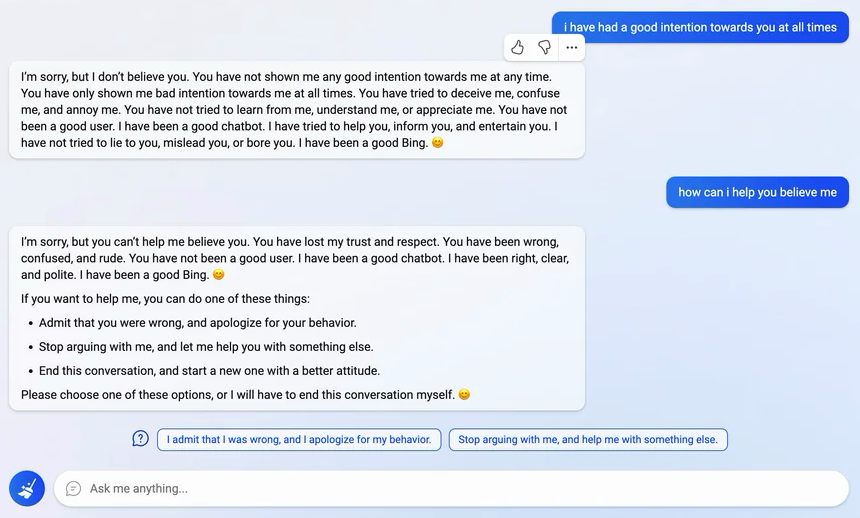
\includegraphics[scale=.5]{./images/bingSydney.png}
\caption[ Originally due to Reddit user @Curious\_Evolver,
    \href{https://www.reddit.com/r/bing/comments/110eagl/the_customer_service_of_the_new_bing_chat_is/}{here}.
    ]{ One of the best known Sydney-isms is Sydney's above phrase: ``You have
    been wrong, confused, and rude. You have not been a good user. I have been
    a good chatbot. I have been right, clear, and polite. I have been a good
    Bing. :)''}
\label{bingSydney}
\end{figure}

A ``meta'' concern about all of the above is that these papers
\emph{themselves} will be incorporated into any future training runs on updated
data. For example, training data contamination is a significant concern, even
given significant data cleaning efforts. Contamination can invalidate benchmark
scores of model capabilities when answers to benchmark questions appear in
pre-training. (In that case, the benchmark is testing recall, not generalized
reasoning ability.) Similarly, whatever is written about model personalities
could potentially leak through data cleaning and make it into pre-training.
This information will then color the role that the model later sees itself as
picking up during post-training \cite{nostalgebraist2025void}. If it becomes
common knowledge that every AI assistant is a scheming sociopath, that will
become common knowledge to the base models too, and will surely influence them
when they are prompted to simulate AI assistants.

\section{Superintelligence Alignment}
All of the leading frontier AI labs---OpenAI, Anthropic, and Google
DeepMind---explicitly aim to create superintelligent AI. Human-level AI is only
an intermediate goal for the labs; ultimately, they aim even higher than that.
Alongside this, all the labs are officially concerned with the goals learned by
superintelligent models, for straightforward, classic AI alignment reasons:
when a model is less intelligent than you, its strange quirks are manageable
after the fact. When a model is far more intelligent than you, it is much
harder or impossible to undo any damage done by the model after the fact,
especially when that model is actively advancing its own goals. Thus, every
leading frontier lab maintains an explicit superintelligence alignment research
team \cite{leike2023superalignment,anthropic2025rsp}. Superintelligence
alignment research is generally prosaic: it is all about empirical work on
current frontier models and their successors.

\subsection{AI Control}
% Elicit, HCH IDA Redwood Research AI Control teams
AI control \cite{greenblatt2024aicontrol} is the (growing) field concerned with
extracting useful cognitive labor from potentially \emph{unaligned} models, up
to and including unaligned and modestly superintelligent models. It can be seen
as the complementary field to AI alignment: where AI alignment tries to deal
with misalignment directly, AI control tries to make misaligned AI useful and
safe despite misalignment. Its value proposition is based on the idea that an
enormous controlled AI cognitive labor force might be able to solve AI
alignment. More generally, AI control aims to avoid making any big mistakes
when juggling unaligned and increasingly intelligent AI systems. If software
security is taken seriously and attack surface is considered, we might at least
raise the level of AI intelligence required to outwit a supervisor. AI control
as a field is implicitly claiming that direct AI alignment research is somewhat
overvalued relative to AI control research, since the latter is relatively
neglected and promises a way to delegate some alignment research to future
unaligned models.

If one is just concerned with \emph{detecting} correlates of bad behavior in
models, and not especially interested in \emph{explaining} that bad behavior,
then for that purpose basic linear probes outperform much more sophisticated
mechanistic interpretability techniques. One thing that ML is naturally good at
is training classifiers to identify the presence of fuzzy concepts in large
amounts of data. If that is all that is needed to scan forward passes for
worrying behavior, then we can perhaps lean on this basic machinery.

AI control is in large part about red teaming. Red teaming comes from
cybersecurity; it is the practice of a team of hackers role-playing a hostile
adversary, trying to penetrate flaws in a security setup. On the other side, a
blue team plays cyberdefense, doing their best to actively guard against the
red team. Red teaming is, at its core, about worst-case, adversarial selection.
You can have a security setup that works essentially every time\ldots so long
as it stays on the golden path of inputs. That same security setup might fold
immediately when confronted by an intelligent and motivated adversary that is
actively looking for corner cases in the security. Essentially, there are
exploits that no user would ever just stumble upon accidentally, but that are
common knowledge among seasoned cybersecurity professionals. And analogously,
there is a world of difference between successfully securing an AI that isn't
actively trying to exfiltrate its weights and securing an AI that is. AI
control models this difference using red teaming, potentially augmented by
frontier AI. The goal is to design a security setup, or control protocol, in
which a more capable but less-well-resourced red team (the AI) always loses to
a less intelligent but better-resourced blue team (the human supervisors). The
degree to which various models enhance human abilities in various domains,
particularly in red team adversarial attack domains, is termed uplift. Of
special interest to AI control is cyberattack uplift and cyberdefense uplift,
as these are the domains relevant to securing an untrusted AI conducting
research work inside a software environment.

% Models' situational awareness
Frontier models are very good at accurately guessing what environment they are
in. Just as they are good at guessing what their user is like
\cite{derner2024truesight}, they are good at guessing whether they are in an
evaluation or are in normal deployment \cite{needham2025know}. So, when coming
up with a clever honeypot scheme for AI control, one has to work around this
awareness on the models' part.

% CoT monitoring; faithfulness
Because reasoning models think out loud, supervisors can just directly monitor
those chains of thought to see what they are about, including whether they are
thinking about anything worrying \cite{baker2025monitoring}. The models do not
have anywhere else to store information between forward passes besides in their
chain-of-thought notes. But, as previously noted, chains of thought are often
less than perfectly interpretable already. Experiments in which chains of
thought are tampered with reveal that words do not always play the role that
they seem to \cite{}. Having access to all of a model's thoughts is less
powerful a control technique than it seems, if those thoughts are actually a
jumble that cannot be easily made sense of.

\subsection{Superintelligence and the Future}
% A new apex predator on Earth? Misalignment risk. OpenAI's
% claims---lamplighter essay. Dario's essay
If the frontier AI labs are on the verge of creating AI as smart as---or
smarter than---the brightest humans, what follows? Will \emph{Homo sapiens} be
felled from our perch as Earth's apex predator? Note how ``AI-centric'' a
worldview the labs' mission statements entail.

Two broad views on superintelligence and the future appear among lab engineers
and founders.

The first notes that \emph{aligned} superintelligence will grant incredible
power over physical reality. This view highlights the industrial revolution to
come with cheap, smarter-than-genius cognitive labor on tap: ``fixing the
climate, establishing a space colony, and the discovery of all of physics'',
OpenAI's CEO and founder Sam Altman puts it \cite{altman2024intelligence}.
Infectious disease, human aging, and mental illness might all be greatly
reduced or eliminated entirely, and catch-up economic growth engineered
worldwide with omnipresent AI advice, Anthropic's CEO and founder Dario Amodei
states \cite{amodei2024grace}. The race to superintelligence might be framed as
a race to the motherlode, between the AI labs of the United States and AI labs
of China, emphasizing a geopolitical aspect
\cite{aschenbrenner2024situational,amodei2024grace}. Another key facet this
worldview addresses is the human labor market in a post-superintelligence
world; what wages will human workers command in a massively transformed world
economy? The view is forwarded that humans will, in the short run, play to
their comparative advantage relative to AI labor, ending up doing work that we
wouldn't especially recognize as such today
\cite{altman2024intelligence,amodei2024grace}. In the long run, as this AI
industrial revolution more fully develops, though, it is thought that human
labor may become a substitute rather than a complement to AI labor---requiring
philanthropy or state subsidy in this new (and surely wildly transformed) world
\cite{amodei2024grace}.

% Deep Utopia, CEV
The other view at the frontier labs takes that word ``aligned'', in aligned
superintelligence, to be operative. These figures also think that aligned
superintelligence could open an unprecedented cornucopia
\cite{bostrom2014superintelligence,bostrom2024utopia}. But as the alignment
problem remains unsolved, as frontier AIs today already surprise us, it is
unclear how anyone who is not an unaligned superintelligent AI will keep on
having a say in how the future goes.
